\documentclass{scrartcl}

\usepackage[ngerman]{babel}
\usepackage[utf8]{inputenc}
\usepackage[T1]{fontenc}
\usepackage{graphicx}
\usepackage{amsmath}
\usepackage{chemmacros}
\usepackage{color}
\usepackage{enumitem}
\usepackage{icomma}
\usepackage{titlesec}
\usepackage{tikz}
\usepackage{adjustbox}
\usepackage{multirow}
\usepackage{upgreek}
\usepackage{url}
\usepackage{wrapfig}
\usepackage{subcaption}
\usepackage{booktabs} 
\usepackage{geometry}
 \geometry{
 a4paper,
 total={170mm,250mm},
 left=20mm,
 top=20mm,
 }

\usepackage[activate={true,nocompatibility},final]{microtype} % better font-rendering
\usepackage[bitstream-charter]{mathdesign} % bitstream font
\titleformat{\section}[hang]{
	\usefont{T1}{bch}{b}{n}\selectfont} % "bch" - Bitstream Character, "b" - bold 
	{} % label
	{0em} % horizontal separation between label and title body
	{\hspace{-0.4pt}\Large \thesection\hspace{0.6em}} % code preceding the title
	[] % additional code following the title body
\titleformat{\subsection}[hang]{
	\usefont{T1}{bch}{b}{n}\selectfont}
	{}
	{0em}
	{\hspace{-0.4pt}\large \thesubsection\hspace{0.6em}}
	[]
\titleformat{\subsubsection}[hang]{
	\usefont{T1}{bch}{b}{n}\selectfont}
	{}
	{0em}
	{\hspace{-0.4pt}\thesubsubsection\hspace{0.6em}}
	[]


\chemsetup{ modules = all }
%\usepackage[version=4]{mhchem}
\chemsetup[redox]{pos=top} % oxid. numbers on top
\usepackage{chemfig}

\newlength{\drop}

\begin{document}
  \begin{titlepage}
    \drop=0.1\textheight
    \centering
    \vspace*{\baselineskip}
    \rule{\textwidth}{1.6pt}\vspace*{-\baselineskip}\vspace*{2pt}
    \rule{\textwidth}{0.4pt}\\[\baselineskip]
    {\LARGE Versuch 1--5 (PSE)\\[0.3\baselineskip] Periodisches System der Elemente}\\[0.2\baselineskip]
    \rule{\textwidth}{0.4pt}\vspace*{-\baselineskip}\vspace{3.2pt}
    \rule{\textwidth}{1.6pt}\\[\baselineskip]
    \scshape
    {Praktische Einführung in die Chemie\par}
    \vspace*{2\baselineskip}
    \vfill
    {\scshape Versuchstag:} \        {\large 21.06.2017}\par
  \end{titlepage}
\section{Theorieteil}
\subsection{Aufbau des Periodensystems der Elemente}
Das Periodensystem der Elemente lässt sich den Zeilen nach in \emph{Perioden} und den Spalten nach in \emph{Gruppen} unterteilen, in denen die Elemente in Reihenfolge aufsteigender \emph{Ordnungszahl} (Kernladungszahl) aufgelistet sind. Den Elementen einer Periode lässt sich eine \emph{Haupquantenzahl} $n$ zuordnen. Die einzelnen Perioden sind zudem anfangend mit der K-Schale alphabetisch benannt. Innerhalb einer Periode sinkt der Atomradius von links nach rechts, da die Kernladung zunimmt und so eine größere Anziehung auf die Elektronen auswirkt. Die Gruppen lassen sich historisch in die Haupt- und Nebengruppen unterteilen, die nach IUPAC-Nomenklatur von 1 bis 18 durchnummeriert sind. Die Elemente einer Gruppe besitzten die gleiche Anzahl an Valenzelektronen, wodurch sie ähnliche Eigenschaften aufweisen. Die Hauptgruppen (also nach IUPAC 1-2, 13-18) heißen: Alkalimetalle, Erdalkalimetalle, Triele, Tetrele, Pentele, Chalkogene, Halogene und Edelgase, während die Nebengruppen (also IUPAC 3-12) bis auf Gruppe 3, die Selten-Erd-Metalle, nach ihrem ersten Element benannt sind.
\subsection{Elektronenkonfiguration der Atome}
Der Zustand der Elektronen eines Atoms lässt sich durch vier \emph{Quantenzahlen} ausdrücken. 
\begin{enumerate}
	\item \textbf{Hauptquantenzahl} $n=1,2,\dots$: Entspricht der Schale, in der sich die Valenzelektronen aufhalten. 
	\item \textbf{Nebenquantenzahl} $l=0,\dots,n-1$: Beschreibt die Anzahl der Unterschalen, die gleich der Hauptquantenzahl $n$ der Schale ist. Die einzelnen $l$ werden mit einem Buchstaben verknüpft, so ist $l=0$ \textbf{s}, $l=1$ \textbf{p}, $l=2$ \textbf{d} und $l=3$ \textbf{f}.
	\item \textbf{magnetische Quantenzahl} $m=-l,\dots,+l$: Jeder Unterschale sind Orbitale zuzuweisen. Die magnetische Quantenzahl $m$ beschreibt die räumliche Anordnung, bzw. Orientierung der Orbitale. 
	\item \textbf{magnetische Spinquantenzahl} $s=\pm\frac{1}{2}$: Jedes Elektron besitzt einen Spin, entweder $+\frac{1}{2}$ oder $-\frac{1}{2}$. Je Orbital können sich maximal zwei Elektronen entgegengesetzen Spins aufhalten. 
\end{enumerate}
\begin{wrapfigure}{r}{.3\textwidth}
	\centering
	\caption{Orbitale im PSE\protect\footnotemark}
	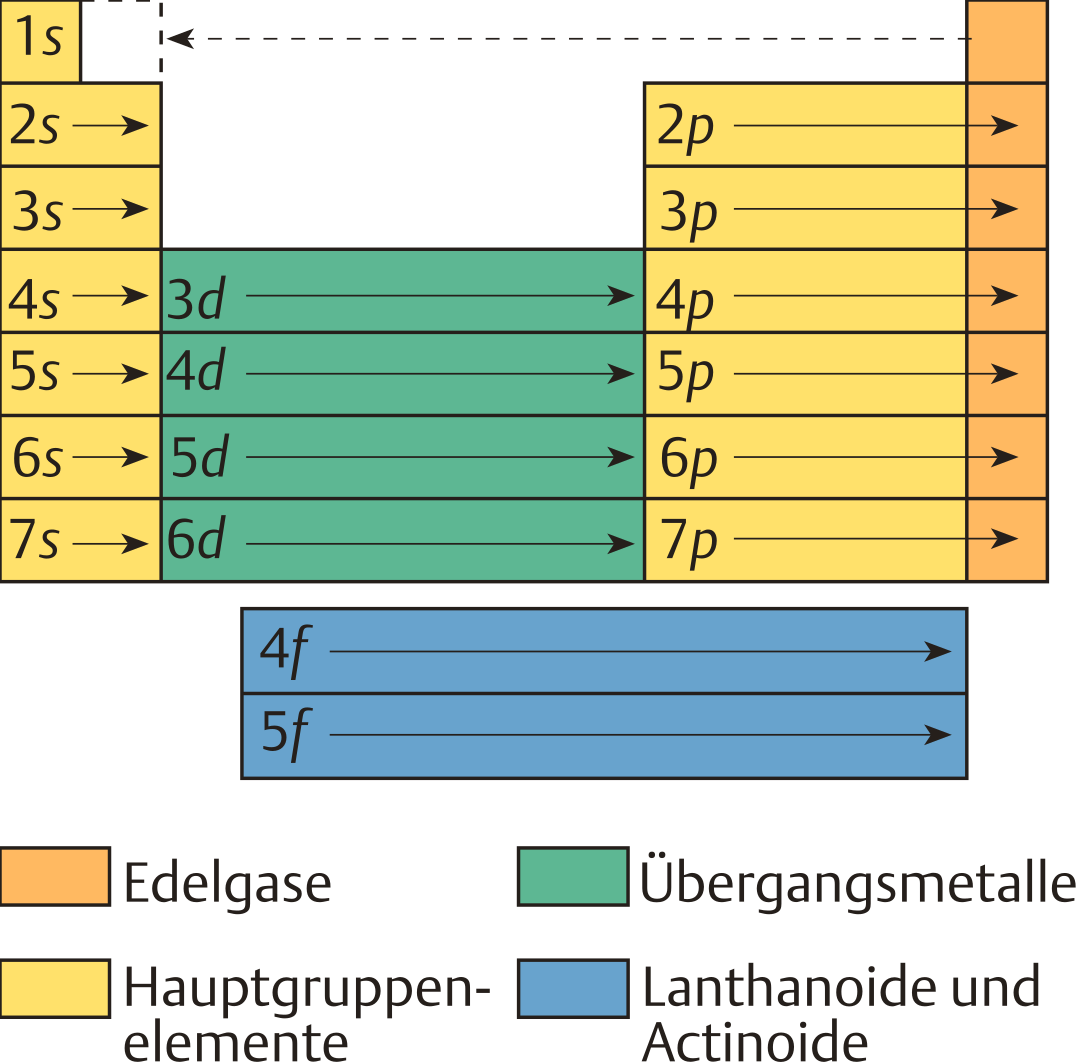
\includegraphics{Aufbauprinzip.png}
\end{wrapfigure}
\footnotetext{Quelle: Basiswissen der Chemie, Mortimer, 12. Auflage, 2015; Seite 91}

	Nach dem \texttt{Pauli-Prinzip} können keine Elektronen eines Atoms in allen vier Quantenzahlen übereinstimmen. Daraus folgt die letzte Aussage, dass für zwei Elektronen, die in $n$, $l$ sowie in $m$ übereinstimmen, also sich in dem selben Orbital aufhalten, notwendigerweise ihre Spins $s$ entgegengerichtet sein müssen. 

	Die Verteilung der Elektronen auf die Orbitale nennt man die \emph{Elektronenkonfiguration}. Die Orbitale werden der geringst möglichen Energie nach aufgefüllt, wobei nach der \texttt{Hund'schen Regel} \emph{entartete} Orbitale, d.h. energiegleichen Orbitale, erst einfach besetzt werden. Generell steigt mit höherem $n$, sowie höherem $l$ die Energie eines Orbitals. Jedoch ist beispielsweise das 4$s$-Orbital bei den meisten Elementen energetisch niedriger als das 3$d$-Orbital und wird somit zuerst besetzt. 
\subsection{Orbitale}
\subsubsection{$s$-Orbital}
Es gibt nur ein $s$-Orbital. Dieses tritt in jeder Periode auf. Es liegt kugelsymmetrisch im Koordinatenursprung und hat keine Knotenfläche. 
\subsubsection{$p$-Orbital}
Es gibt drei verschiedene $p$-Orbitale, die jeweils eine Knotenfläche im Koordinatenursprung haben. Hier ist die Aufentaltswahrscheinlichkeit der Elektronen null. Man bezeichnet die Orbitale typischerweise nach der Achse an der entlang sie ausgerichtet sind.
\begin{figure}[h]
	\centering
	\caption{Grenzflächendiagramme der drei $p$-Orbitale\protect\footnotemark}
	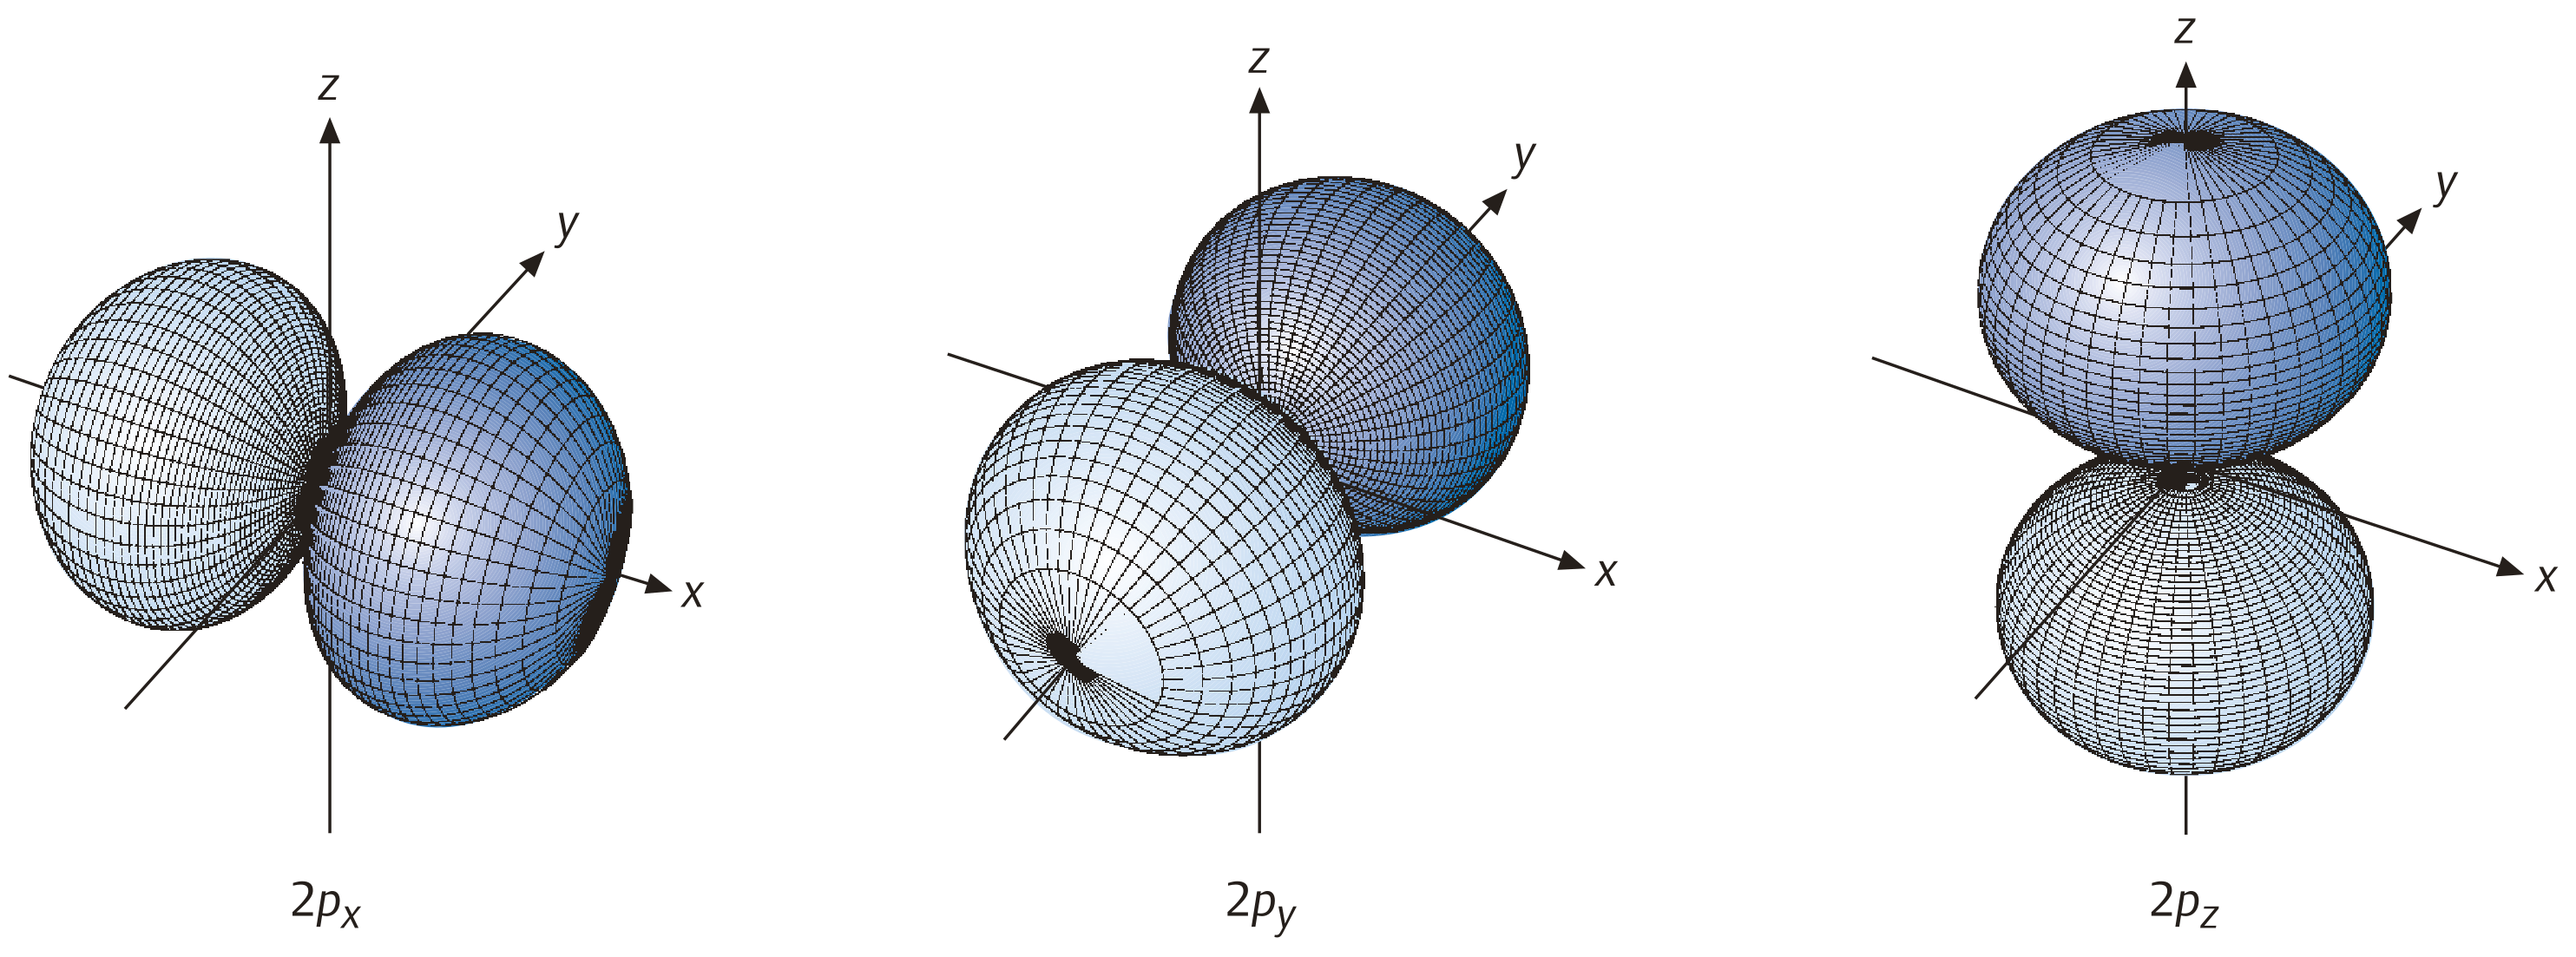
\includegraphics[scale=.75]{p-Orbitale.png}
\end{figure}
\footnotetext{Quelle: Basiswissen der Chemie, Mortimer, 12. Auflage, 2015; Seite 86} 
\subsubsection{$d$-Orbitale}
Es git fünf verschiedene $d$-Orbitale, die alle zwei Knotenflächen im Koordinatenursprung aufweisen. Drei davon, $d_{xy}, d_{xz}, d_{yz}$ liegen jeweils zwischen den zwei Achsen, nach denen sie benannt werden. Das $d_{x^2-y^2}$-Orbital hat wie die drei zuvor vier Lappen, diese liegen jedoch auf der x und y Achse. Das fünfte $d_{z^2}$-Orbital hat nur 3 Lappen, zwei davon hantelförmig entlang der z-Achse und ein Lappen torusförmig in der x-y Ebene.  
\begin{figure}[h]
	\centering
	\caption{Grenflächendiagramme der fünf $d$-Orbitale\protect\footnotemark}
	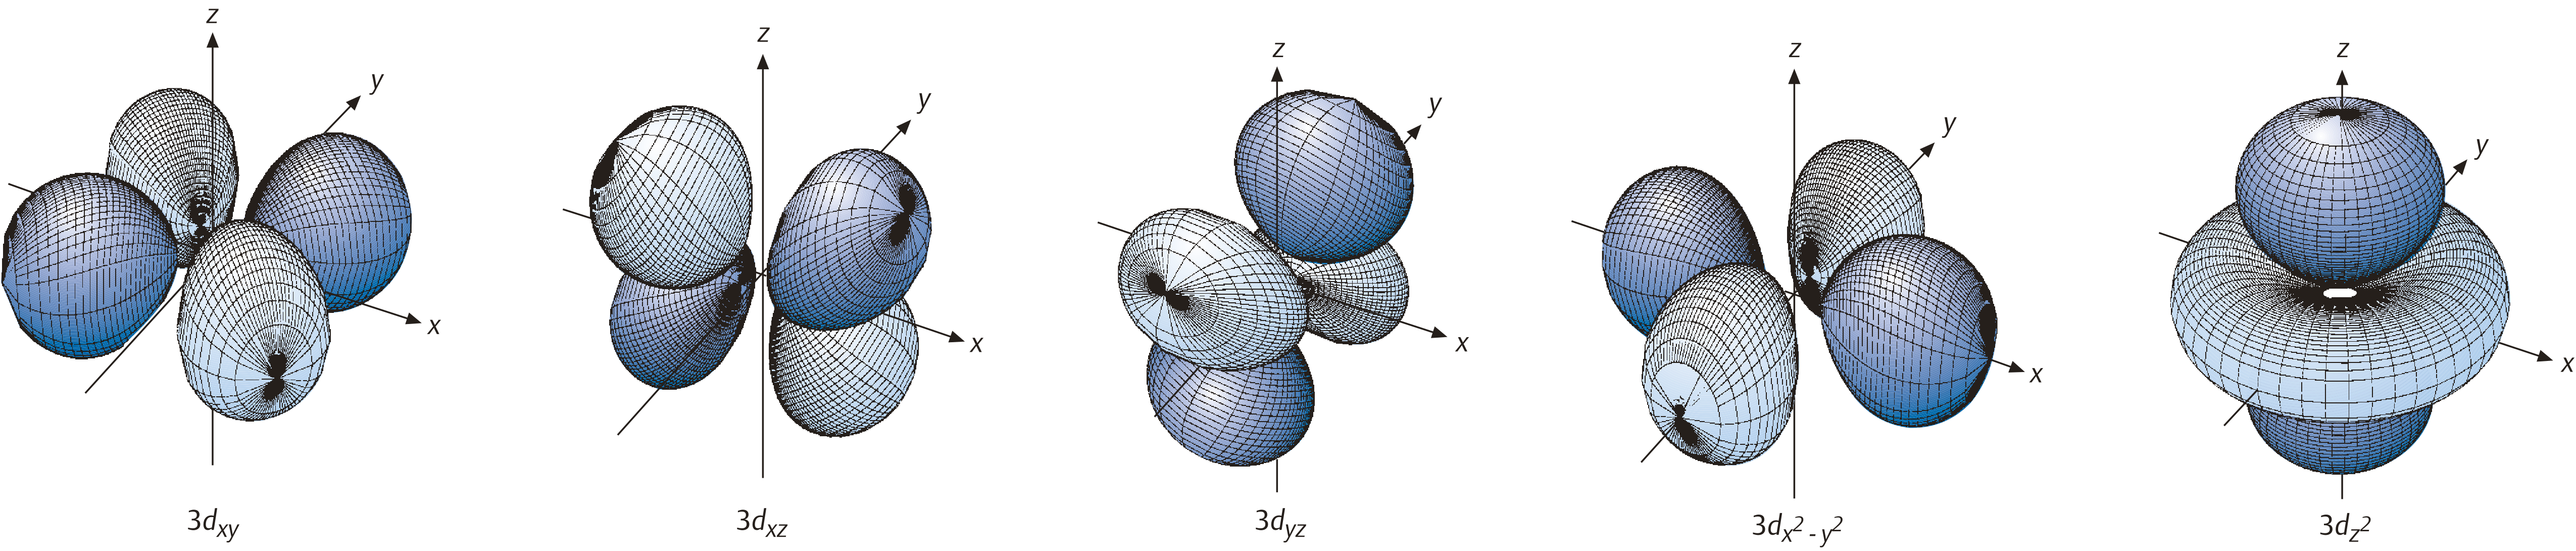
\includegraphics[width=\textwidth]{d-Orbitale2.png}
\end{figure}
\footnotetext{Quelle: Basiswissen der Chemie, Mortimer, 12. Auflage, 2015; Seite 87}
\subsection{Das HSAB-Prinzip}
Das HSAB-Prinzip (\textbf{H}ard and \textbf{S}oft \textbf{A}cids and \textbf{B}ases) beschreibt die Bindungen von Lewis-Säuren und -Basen. Unter \emph{harten} Lewis-Säuren oder -Basen versteht man Teilchen, die einen kleinen Radius, eine hohe Ladungsdichte und kaum polarisierbar sind. \emph{Weiche} Lewis-Säuren/-Basen sind hingegen solche, die einen großen Radius, eine geringe Ladungsdichte und leicht polarisierbar sind. Nach dem \texttt{Pearson-Konzept} sind Verbindungen zwischen jeweils harten Säuren und harten Basen, sowie zwischen jeweils weichen Säuren und weichen Basen stabil, während Kreuzungen wie harte Säure/Base mit weicher Base/Säure eher instabil sind. 
\section{Versuche}
 \subsection{Löslichkeit von Silberhalogeniden}
\subsubsection{Aufgabenstellung}
Bei diesem Versuch soll das Löslichkeitsverhalten von Silberhalogeniden untersucht werden.
\subsubsection{Versuchsdurchführung}
Zu erst wurden Lösungen von KCl, KBr und KI hergestellt, indem eine Spatelspitze des jeweiligen Stoffes in ein Reagenzglas gefüllt wurde und dann mit ca. 2 cm dem. Wasser befüllt wurde. Diese Lösung wurde dann mit \ch{AgNO3}-Lösung versetzt. Nun wurde eine \ch{(NH4)2CO3}-Lösung erstellt (gelöst in Wasser) und dazu gegeben und beobachtet ob sich der gebildete Niederschlag wieder auflöst. Dieser Vorgang wurde dann mit konz. Ammoniaklösung wiederholt und beobachtet.
\subsubsection{Beobachtung}
Nachdem die Ausgangsmaterialien mit \ch{AgNO3} versetzt wurden, war bei KCl ein weißer Niederschlag, bei KBr ein leicht gelber und bei KI ein gelber Niederschlag zu beobachten.
Nach Zugabe von \ch{(NH4)2CO3} kann keine Veränderung des Niederschlages beobachtet werde. Gibt man jedoch konz. Ammoniaklösung dazu, kann bei KCl und KBr ein auflösen des Niederschlages beobachtet werden, wo in gegen dazu bei der alten KI-Lösung nichts passierte.
\subsubsection{Auswertung}
Nach Zugabe von Wasser zum Ausgangsstoff dissoziieren diese wie folgt:\\ 
\ch{KCl + H2O <=> K^+ + Cl^-}\\
\ch{KBr + H2O <=> K^+ + Br^-}\\
\ch{KI + H2O <=> K^+ + I^-}\\ 
Diese reagieren dann mit der \ch{AgNO3}-Lösung weiter, welche zu erst auch dissoziiert:\\ 
\ch{AgNO3 + H2O <=> Ag^+ + NO3^-}\\ \\ 
\ch{Cl^- + Ag^+ <=> AgCl}\\
\ch{Br^- + Ag^+ <=> AgBr}\\
\ch{I^- + Ag^+ <=> AgI}

Gibt man die \ch{(NH4)2CO3}-Lösung dazu, entsteht zu ganz kleinen Teilen ein Silberdiamminkomplex, jedoch entsteht nicht genügend \ch{NH3} bei der Dissoziation um den Feststoff aufzulösen.\\
Dissoziation von \ch{(NH4)2CO2}:\\ 
\ch{(NH4)2CO3 +H2O <=> 2NH4^+ + CO3^{2-}}\\
\ch{NH4^+ + H2O <=> NH3 + H3O^+}\\
\ch{CO3^{2-} + H2O <=> HCO3^- + OH^-}\\
\ch{HCO3^- + H2O <=> H2CO3 + OH^-}\\
\ch{H2CO3 <=> CO2 + H2O}

Gibt man jetzt die Ammoniaklösung hinzu entsteht ein Silberdiamminkomplex. Da die Reaktionen alles Gleichgewichtsreaktionen sind, muss nach dem Prinzip von Le-Chatelier ein Silberion in Lösung gehen und somit löst sich der Feststoff auf. Dies ist nur bei AgCl und bei AgBr der Fall, bei AgI bleibt der Feststoff unverändert.\\ \\
\ch{Ag^+ + NH3 <=> [Ag(NH3)2]^+}
\subsubsection{Löslichkeitsprodukt}
Das Löslichkeitsprodukt\footnote{Quelle: \url{http://www.chemieunterricht.de/dc2/komplexe/silber.html}} von den drei Silberhalogeniden beträgt:\\ 
K\textsubscript{L}(AgCl) = 1,7 $\cdot$ 10\textsuperscript{-10} $\frac{\text{mol}^2}{\text{l}^2}$\\
K\textsubscript{L}(AgBr) = 5,0 $\cdot$ 10\textsuperscript{-13} $\frac{\text{mol}^2}{\text{l}^2}$\\
K\textsubscript{L}(AgI) = 8,5 $\cdot$ 10\textsuperscript{-17} $\frac{\text{mol}^2}{\text{l}^2}$
\subsubsection{Periodische Eigenschaften von Halogenen}
Elementare Halogene liegen in zweiatomigen Molekülen vor, wie zB. F\textsubscript{2} oder Cl\textsubscript{2}. Halogene wie auch ihre zweiatomige Moleküle sind sehr reaktionsfreudig und reagieren heftig, wobei die Stärke der Reaktion von Fluor zu Iod abnimmt, wie auch die Elektronegativität. Dagegen nehmen Dichte, Siede- und Schmelzpunkt auf Grund der zunehmenden Molmasse nach unten hin zu.


 
\subsection{pH-Werte von Hydroxiden der dritten Hauptgruppe}
\subsubsection{Aufgabenstellung} 
Es wurden die pH Werte der Hydroxide bzw. Oxid-Hydroxide der ersten sieben Elemente der dritten Periode bestimmt und die Veränderung dieser beim Übergang von Metallen zu Nichtmetallen beobachtet.


\subsubsection{Durchführung} 
Die pH-Werte wurden für folgende sieben Verbindungen bestimmt: \ch{NaOH}, \ch{Mg(OH)2}, \ch{Al(OH)3}, \ch{Si(OH)4}, \ch{PO(OH)3}, \ch{SO2(OH)2} und \ch{ClO3(OH)}. Dazu wurden bei festen Verbindungen jeweils eine Spatelspitze in ein Reagenzglas gegeben und dieses anschließend bis zur Hälfte mit demineralisiertem Wasser aufgefüllt. Bei flüssigen Verbindungen wurde das Reagenzglas erst zur Hälfte mit demineralisiertem Wasser befüllt und dann jeweils 3-5mm hoch die entsprechende Verbindung hinzugegeben.
Nun wurde der pH-Wert mit Indikatorpapier bestimmt (es wurde mit einem Stab betupft um Material zu sparen).


\subsubsection{Beobachtung}
Für die Stoffe ergaben sich folgende pH-Werte und Farben:
\begin{figure}[h]
	\centering
	\caption{Gelöste Stoffe, ihr \pH-Wert und ihre Farbe}
	\begin{tabular}{l c c}
		\toprule
		Stoff & \pH-Wert & Farbe \\ \midrule
		\ch{NaOH} & 10 & dunkelgrün \\
		\ch{Mg(OH)2} & 8 & \--- \\
		\ch{Al(OH)3} & 8 & \--- \\
		\ch{Si(OH)4} & 7 & \--- \\
		\ch{PO(OH)3} & 2-3 & rot \\
		\ch{SO2(OH)2} & 0-1 & lila \\
		\ch{ClO3(OH)} & 0-1 & lila  \\
		\bottomrule
	\end{tabular}
\end{figure}
\subsubsection{Auswertung}
Dissoziationsgleichungen nach steigender Ordnungszahl
\begin{itemize}
	\item\ch{NaOH <=>>[ H2O ] Na^+ + OH^-}
	\item\ch{Mg(OH)2 <=>[ H2O ] Mg^2+ + 2OH^-}
	\item\ch{Al(OH)3 <<=>[ H2O ] Al^3+ + 3OH^-}
	\item\ch{Si(OH)4 <<=>[ H2O ] SiO^4- + 4H^+}
	\item\ch{PO(OH)3 <=>>[ H2O ] PO4^3- + 3H^+}
	\item\ch{SO2(OH)2 <=>>[ H2O ] SO4^2- + 2H^+}
	\item\ch{ClO3(OH) <=>>[ H2O ] ClO4^- + H^+}
\end{itemize}
Man sieht anhand der Dissoziationsgleichungen, dass von Natriumhydroxid bis Aluminiumhydroxid Hydroxid-Ionen bei der Dissozation der entstehen, dass bedeutet, dass diese Stoffe basisch sind. Da sich jedoch das Gleichgewicht von Natrium nach Aluminium von der Produkt- auf die Eduktseite verlagert, werden die pH-Werte kleiner.
Ab Siliciumhydroxid werden jedoch Protonen bei der Dissoziation frei, d.h. dass diese Stoffe sauer sind. Da sich hier Richtung Perchlorsäure das Gleichgewicht wieder auf die Produktseite verlagert werden auch hier die pH-Werte immer kleiner.
Der Übergang von basisch zu sauer liegt am Übergang von Metall zu Nichtmetall. Die Metalle bilden in Wasser Basen die Nichtmetalle Säuren. Dies liegt daran, dass innerhalb der Periode die Elektronegativität zunimmt. Silicium und aufwärts sind so Elektronegativ, dass es ihnen nicht möglich ist die zur neutral Ladung nötige Menge an Hydroxid zu binden. Anstattdessen wird Sauerstoff benutzt um Hydroxid anlagern zu können, was eine sauere Wirkung hervorruft.
Die zunehmende Elektronegativität innerhalb der Periode ist auch dafür verantwortlich, dass innerhalb der Metalle und Nichtmetalle der pH-Wert abnimmt. Innerhalb der Metalle wird die Bindung des negativen \ch{OH^-} immer stärker beziehungsweise innerhalb der Nichtmetalle die Bindung des positiven \ch{H^+}immer schwächer.
Auf dem Tablett war nur \ch{SiO2} vorhanden, da \ch{Si(OH)4} nicht in Glas gelagert werden kann. Dies ist aber unproblematisch, da \ch{Si(OH)4} entsteht wenn man \ch{SiO2} in Wasser gibt.

\subsection{Vergleich der Farbigkeit von Übergangsmetallkomplexen/-verbindungen mit Haupt-gruppenmetallkomplexen/-verbindungen}
\subsubsection{Aufgabenstellung}
Der Versuch soll die Farbigkeit und deren Entstehung bei Verbindungen von Übergangsmetallen und anaologen Hauptgruppenmetallverbindungen vergleichen.
\subsubsection{Durchführung}
Im ersten Versuchsteil wurden vier Verbindungen vorbereitet: \ch{KCl}, \ch{CaCl2}, \ch{FeCl3} und \ch{CuSO4}. Dazu wurde jeweils eine Spatelspitze in ein Reagenzglas gegeben und das Reagenzglas dann zu einem Viertel mit demineralisiertem Wasser befüllt.
Anschließend wurde die Farbe dokumentiert. Daraufhin wurden die Lösungen 2 cm hoch mit Ammoniak versetzt und Farbänderungen und Niederschläge nach dem setzten dokumentiert.

Im zweiten Versuchsteil wurden nach gleichem Vorgehen folgende vier Lösungen hergestellt: \ch{K2SO4}, \ch{K2CrO4}, \ch{KClO4} und \ch{KMnO4}.
Es werden nun die Farben ohne Zugabe weiterer Stoffe notiert.
\subsubsection{Beobachtung}
\begin{figure}[h]
	\centering
	\caption{Beobachtung erster und zweiter Versuchsteil}
	\begin{subfigure}{\textwidth}
		\centering
	\caption{Stoffe und ihre Farbe in Lösung}
	\begin{tabular}{l l l}
		\toprule
		Stoffe & Farbe in wässriger Lösung & mit Ammoniaklösung \\ \midrule
		\ch{KCl} & durchsichtig & durchsichtig \\
		\ch{CaCl2} & durchsichtig & durchsichtig \\
		\ch{FeCl3} & orange/kupferbraun & kräftig bräunlich, rostfarben \\
		\ch{CuSO4} & durchsichtig, leicht bläulich & tief blau \\
		\bottomrule
	\end{tabular}
	\vspace*{1cm}
	\end{subfigure}
	\begin{subfigure}{\textwidth}
	\centering
	\caption{Stoffe und ihre Farbe in wässriger Lösung}
	\begin{tabular}{l l}
		\toprule
		Stoffe & Farbe in wässriger Lösung \\ \midrule
		\ch{K2SO4} & durchsichtig \\
		\ch{K2CrO4} & gelb \\
		\ch{KClO4} & durchsichtig, leicht gelb \\
		\ch{KMnO4} & lila \\
		\bottomrule 
	\end{tabular}
\end{subfigure}
\end{figure}

\section{Literatur}
\begin{enumerate}[label=(\arabic*)]
	\item \emph{Praktische Einführung in die Chemie
für Studierende der Fachrichtungen
Technische Biologie und Physik}. Praktikumsskript, Universität Stuttgart,
SoSe 2017.  
	\item Prof. Dr. D. Gudat. \emph{„Einführung in die Chemie für Naturwissenschaftler“}. Vorlesungsskript
	\item \emph{Das Basiswissen der Chemie}. Charles E. Mortimer, Ulrich Müller. 12. Auflage, 2015
\end{enumerate}
\end{document}		
